\documentclass[12pt, a4paper]{article}
\usepackage{../../../myconfig_line} % Gọi file cấu hình từ ngoài gốc vào
% ==========================================
% BẮT ĐẦU NỘI DUNG TÀI LIỆU
% ==========================================
\begin{document}

% Truyền 3 tham số: {Nhãn cam} {Chữ to chính giữa} {Chữ ở góc phải Header}
\titlebox{Chủ đề: Tích phân}{Tốc dộ thay đổi đại lượng và lượng tích lũy}{Thay đổi đại lượng}

\drawdashlines{29}

%--- CÂU 1 ---
\questionShortAnswer{30}{1}{Ở giai đoạn thải trừ, giai đoạn cuối sau khi một người uống một liều thuốc, nồng độ thuốc trong máu, ký hiệu là \(C(t)\) (đơn vị: mg/l), giảm dần sau \(t\) giờ kể từ khi giai đoạn này bắt đầu. Khi đó, tốc độ giảm nồng độ \(C'(t)\) tỉ lệ với chính nồng độ hiện có, tức là: \(\dfrac{C'(t)}{C(t)} = -k\) (\(k\) là một hằng số dương). Biết rằng khi bắt đầu giai đoạn thải trừ, nồng độ thuốc còn lại là 12 mg/l và sau 6 giờ kể từ lúc bắt đầu thải trừ, nồng độ đo được là 3 mg/l. Sau khoảng bao nhiêu giờ thì nồng độ còn lại bằng 2 mg/l? (kết quả làm tròn đến hàng phần mười).}

% --- CÂU 2 ---
\questionShortAnswer{32}{2}{Một bể chứa nước hình trụ thẳng đứng đang đầy nước. Khi mở nút xả ở đáy, nước chảy ra ngoài với tốc độ giảm thể tích tỉ lệ thuận với căn bậc hai chiều cao mực nước hiện tại trong bể. Nếu gọi \(V(t)\) là thể tích nước còn lại trong bể sau \(t\) phút, tốc độ thay đổi thể tích được mô tả bởi \(V'(t) = -k\sqrt{V(t)}\), với \(k > 0\). Biết bể ban đầu có 144 lít nước. Sau 10 phút xả, lượng nước còn lại là 64 lít. Hỏi sau bao nhiêu phút kể từ lúc mở nút xả thì bể cạn hoàn toàn?}

\drawdashlines{29}

% --- CÂU 3 ---
\questionShortAnswer{23}{3}{Một cái chậu đựng nước có dạng hình chóp cụt đều, đáy chậu là tam giác đều cạnh bằng 2 dm, miệng chậu là tam giác đều cạnh bằng 5 dm và chiều cao chậu nước bằng 3 dm. Người ta bơm nước vào chậu với lưu lượng không đổi \(\dfrac{\sqrt{3}}{3}\) lít/phút. Tại thời điểm 14 phút sau khi bơm tốc độ dâng lên của nước trong chậu là \(\dfrac{1}{a}\) dm/phút, giá trị của \(a\) bằng bao nhiêu?
\begin{figure}[H]
    \centering
    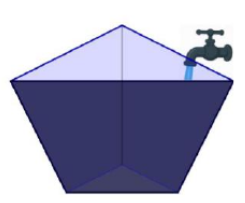
\includegraphics[width=0.3\textwidth]{../images/chopcut3.png}
\end{figure}
}

% --- CÂU 4 ---
\questionShortAnswer{23}{4}{Một chiếc đồng hồ cát nghệ thuật bằng thủy tinh có bầu chứa phía trên và bầu chứa phía dưới bằng nhau, bên trong chứa một chất lỏng đặc biệt. Khi bầu phía trên chứa đầy chất lỏng, thể tích chất lỏng bên trong đúng bằng thể tích của một khối tròn xoay sinh ra khi quay quanh trục \(Ox\) hình phẳng giới hạn bởi đồ thị hàm số \(y = 2\sqrt{x}\), trục hoành và hai đường thẳng \(x = 0, x = 9\). Các đơn vị trên hệ trục tọa độ được tính bằng centimet. Cổ hẹp xem như không đáng kể. Ban đầu, bầu chứa phía trên đầy chất lỏng. Khi bắt đầu tính giờ, chất lỏng chảy qua cổ hẹp xuống bầu chứa phía dưới với tốc độ không đổi và chảy hết trong đúng 27 phút. Trong suốt quá trình chảy, bề mặt trên của chất lỏng luôn là một mặt phẳng nằm ngang. Gọi \(h\) là chiều cao của khối chất lỏng còn lại trong bầu phía trên tại thời điểm \(t\), tính từ cổ hẹp hướng lên trên dọc theo trục \(Ox\). Hỏi sau bao nhiêu phút kể từ lúc bắt đầu chảy, chiều cao khối chất lỏng còn lại trong bầu phía trên đúng 3 cm?
\begin{figure}[H]
    \centering
    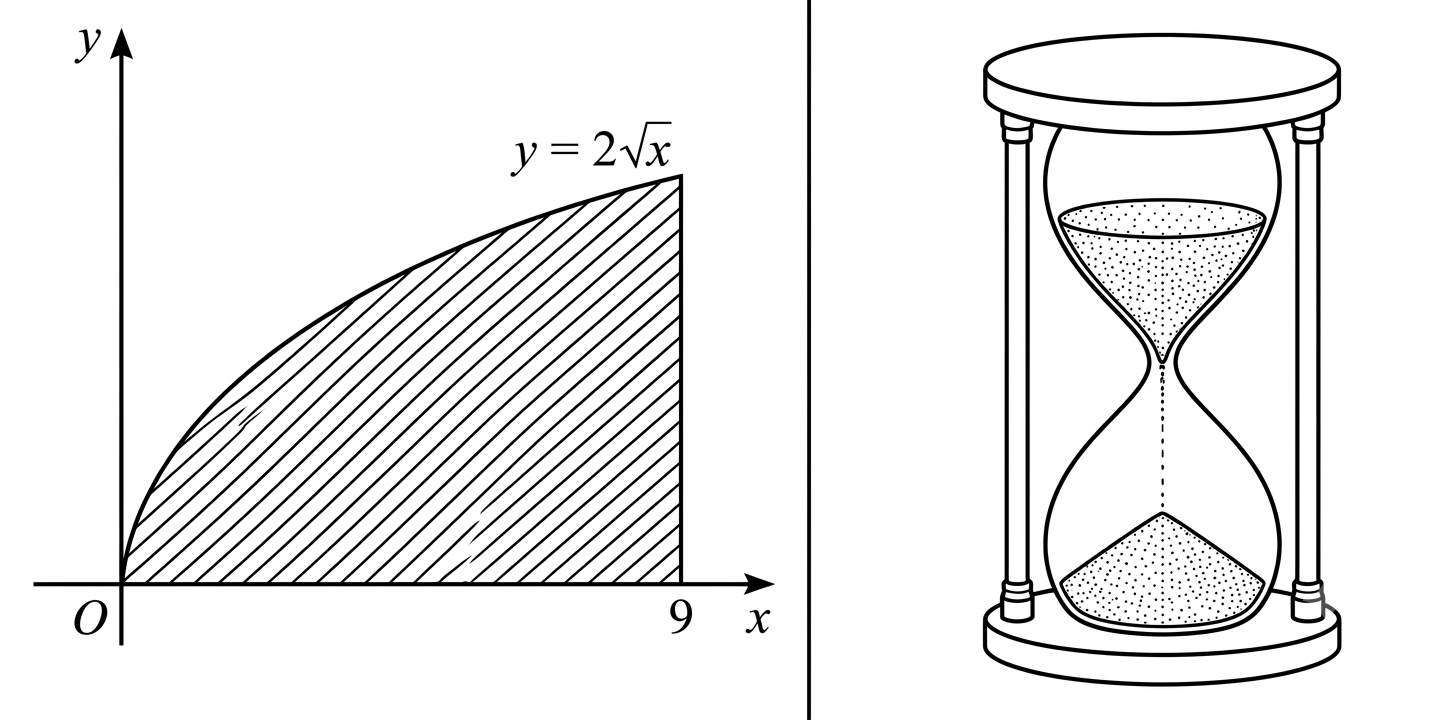
\includegraphics[width=0.4\textwidth]{../images/DHcat.png}
\end{figure}
}

\drawdashlines{29}

% --- CÂU 5 ---
\questionShortAnswer{30}{5}{Nhiệt độ trung bình của Trái Đất có xu hướng tăng do sự gia tăng nồng độ \(CO_2\) trong khí quyển. Giả sử nồng độ \(CO_2\) trong khí quyển (tính bằng ppm - parts per million) được mô tả bởi hàm số \(C(t) = 420 + 2,5t + 0,02t^2\), trong đó \(t\) được tính theo năm và \(t = 0\) ứng với năm 2025. Mối quan hệ giữa độ tăng nhiệt độ trung bình toàn cầu \(T(t)\) (đơn vị: \(^\circ C\)) và nồng độ \(CO_2\) được mô tả như sau: \(T(t) = \displaystyle\int_{0}^{t} kC(x)dx\) với \(k\) là hằng số. Nếu không có biện pháp giảm phát thải \(CO_2\) và giả sử nhiệt độ trung bình của Trái Đất tăng thêm \(0,99^\circ C\) từ năm 2025 đến năm 2040 thì nhiệt độ trung bình của Trái Đất tăng thêm bao nhiêu \(^\circ C\) từ năm 2025 đến năm 2060? (làm tròn kết quả đến hàng phần trăm).
}

% --- CÂU 6 ---
\questionShortAnswer{28}{6}{Trong một chương trình giao lưu âm nhạc đón tết vui xuân, ban đầu với sự tham dự của 2100 khán giả. Ban tổ chức đã thống kê số lượng khán giả ở lại sân khấu xem âm nhạc theo thời gian, được mô tả bởi một hàm số liên tục theo \(t \in [0; +\infty)\):
\[
f'(t) = \begin{cases}
2100 - 400t, & 0 \leq t \leq 3 \\
a(t-3)^2 + b, & t > 3
\end{cases}
\]
(trong đó \(f'(t)\) là số khán giả, \(t\) là số giờ kể từ khi chương trình bắt đầu, \(a, b\) là tham số thực), với hàm số \(f(t)\) mô tả tổng sự hiện diện của khán giả theo thời gian \(t\). Sau 3 giờ 30 phút số lượng khán giả ở lại sân khấu là 875. Hỏi từ khi bắt đầu cho đến khi khán giả ra về hết, trung bình mỗi giờ còn bao nhiêu khán giả ở lại tham gia chương trình âm nhạc?
}

\drawdashlines{29}

% --- CÂU 7 ---
\questionShortAnswer{20}{7}{Trong một mô hình kinh tế, hàm cung \(y = S(x)\) là giá của một sản phẩm khi nhà sản xuất sẵn sàng bán ra \(x\) sản phẩm, hàm cầu \(y = D(x)\) là giá của một sản phẩm khi người tiêu dùng có nhu cầu mua \(x\) sản phẩm. Điểm cắt nhau \((x_0; y_0)\) của đồ thị hàm cầu và hàm cung được gọi là điểm cân bằng thị trường. Các nhà kinh tế gọi thặng dư tiêu dùng là diện tích của hình giới hạn bởi đồ thị hàm cầu, đường ngang \(y = y_0\) và trục tung. Tương tự, thặng dư sản xuất là diện tích của hình giới hạn bởi đồ thị của hàm cung, đường ngang \(y = y_0\) và trục tung. Xét thị trường tấm pin năng lượng mặt trời thế hệ mới, hàm cầu là \(p = D(x) = 4 - 0,2x\) triệu đồng/tấm. Hàm cung là \(p = S(x) = 0,4 + 0,1x + \dfrac{1}{m}x^2\) triệu đồng/tấm, với \(m > 0\). Biết rằng tại trạng thái cân bằng thị trường, thặng dư sản xuất đạt được là 4,2 tỷ đồng. Tại thời điểm này, thặng dư tiêu dùng là bao nhiêu tỷ đồng?
\begin{figure}[H]
    \centering
    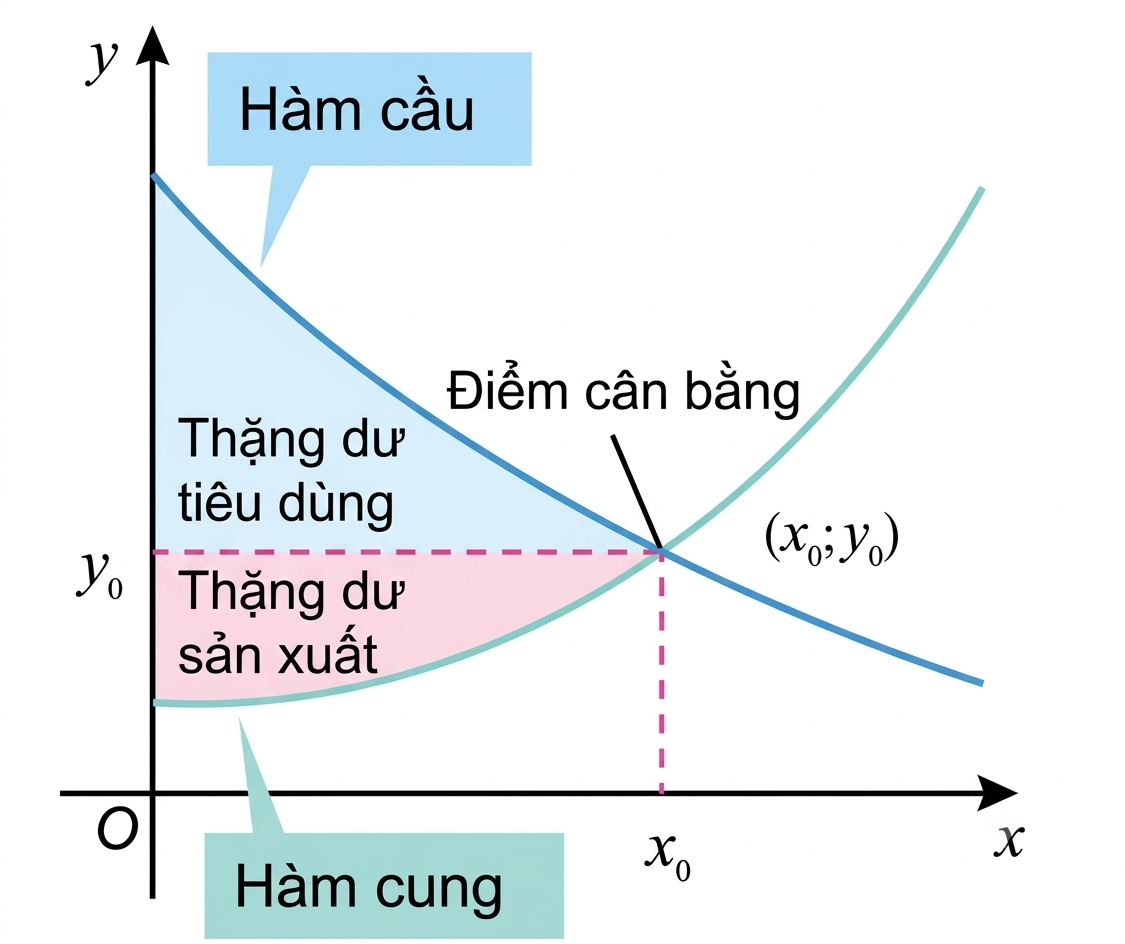
\includegraphics[width=0.4\textwidth]{../images/CungCau.png}
\end{figure}
}

% --- CÂU 8 ---
\questionShortAnswer{30}{8}{Một gia đình sản xuất chiếu cói ở Nga Sơn mỗi ngày sản xuất được \(x\) chiếc chiếu (\(0 \leq x \leq 20\)). Chi phí biên để sản xuất \(x\) chiếc chiếu (tính bằng nghìn đồng) cho bởi hàm số sau: \(C'(x) = 3x^2 - 4x + 10\). Biết rằng chi phí cố định ban đầu để sản xuất là 500 nghìn đồng. Giả sử gia đình này bán hết chiếu mỗi ngày với giá 270 nghìn đồng/chiếc chiếu. Tính lợi nhuận tối đa theo đơn vị nghìn đồng mà gia đình đó thu được?
}

\drawdashlines{29}

















\end{document}